\documentclass{article}
\title{Blanchard Ch.3}
\author{Dawei Wang}
\date{\today}
\usepackage{ctex}
\usepackage{amsmath}
\usepackage{amssymb}
\usepackage{graphicx} %插入图片的宏包
\usepackage{float} %设置图片浮动位置的宏包
\usepackage{subfigure} %插入多图时用子图显示的宏包
\begin{document}
	\maketitle
\section{GDP的构成}
\[
GDP=C+I+G+NX
\]


C:消费者购买物品和劳务的支出。

\hspace*{\fill}

I:也称为固定资产投资(区分于存货投资),固定资产投资包括非住宅投资(公司购置新厂房和机器)和住宅投资。

经济学家的投资专指购买新的资本物品如厂房、机器设备。对于股票和其他金融资产的投资叫作“金融投资”。

\hspace*{\fill}

G:政府对物品或劳务(公务员工资)的购买,不包括转移支付、政府债务利息支出。

\hspace*{\fill}

NX:净出口=出口-进口。

国外消费者、企业和政府购买国内的物品和劳务-国内消费者、企业和政府购买国外的物品和劳务。

\hspace*{\fill}

库存投资(inventory investment):生产的-售出的(没卖出去的叫作库存投资)。存货并不是需求的一部分。


\section{商品需求}
用Z代表商品的总需求,可以把Z写成如下形式:

\[
Z\equiv C+I+G+X-IM
\]

假设(简化):

1. 只考虑产品市场;

2. 假设产品的价格水平P固定;

3. 假设该经济体是封闭的:进口和出口均为0。
\[
Z\equiv C+I+G
\]

\subsection{消费(C)}
决定消费的最主要的是可支配收入($ Y_D , disposable\enspace income$):消费者从政府那里获取转移支付并扣除税收之后的收入。
\[
C=c_0+c_1Y_D
\]
$ c_0 $:自主消费($ c_0>0 $);$ c_1 $:边际消费倾向($ 0<c_1<1 $)。

\hspace*{\fill}

可支配收入:
\[
Y_D\equiv Y-T
\]
其中T为政府税收-政府转移支付。

因此消费函数为:
\[
C=c_0+c_1(Y-T)
\]

\subsection{投资(I)}
此处将投资当作外生变量来处理(内生变量——由模型解释,外生变量——给定的):
\[
I=\overline{I}
\]

\subsection{政府支出(G)}
G和T一起反映了财政政策(fiscal policy)——政府可以做出税收和支出的选择。将G和T作为外生变量来处理(作为外生变量的原因是把它们当作政府选择的变量)。

\section{均衡产出决定}

P.S.:

\[
Z=c_0+c_1(Y-T)+\overline{I}+G
\]
产品市场均衡条件(在没有库存的条件下):
\[
Y=Z
\]
因此:
\[
Y=c_0+c_1(Y-T)+\overline{I}+G
\]

\hspace*{\fill}

P.S.:如果企业持有库存,生产就不一定需要等于需求才能使产品市场达到均衡。例如,企业可以动用库存来满足需求的增长,即持有负的存货投资。如果需求减少,企业继续生产积累存货,即持有正的存货投资。

三类等式:恒等式、行为等式、均衡条件。

在均衡条件下,生产Y(等式左边)等于需求(等式右边)。反过来,需求取决于收入Y,收入本身就等于生产。

由于我们既能从生产的角度考虑GDP,又能从收入的角度考虑GDP。故生产和收入是恒等的。


\subsection{代数方法}
\[
Y=c_0+c_1(Y-T)+\overline{I}+G
\]
解得:
\[
Y=\frac{1}{1-c_1}[c_0+\overline{I}+G-c_1T]
\]
其中:$ [c_0+\overline{I}+G-c_1T] $为自主性支出(物品需求不依赖于产出的部分,autonomous spending,不一定为正)。

$ \frac{1}{1-c_1} $为乘数(multiplier),乘数效应:产出变化大于自主支出的直接影响。

乘数效应的来源描述:$ c_0 $增加需求增加,需求增加导致产量增加,产量增加导致收入同等增加。收入增加进一步增加消费,从而进一步增加需求。等等。





\subsection{图形方法}

\begin{figure}[H] %H为当前位置,!htb为忽略美学标准,htbp为浮动图形
	\centering %图片居中
	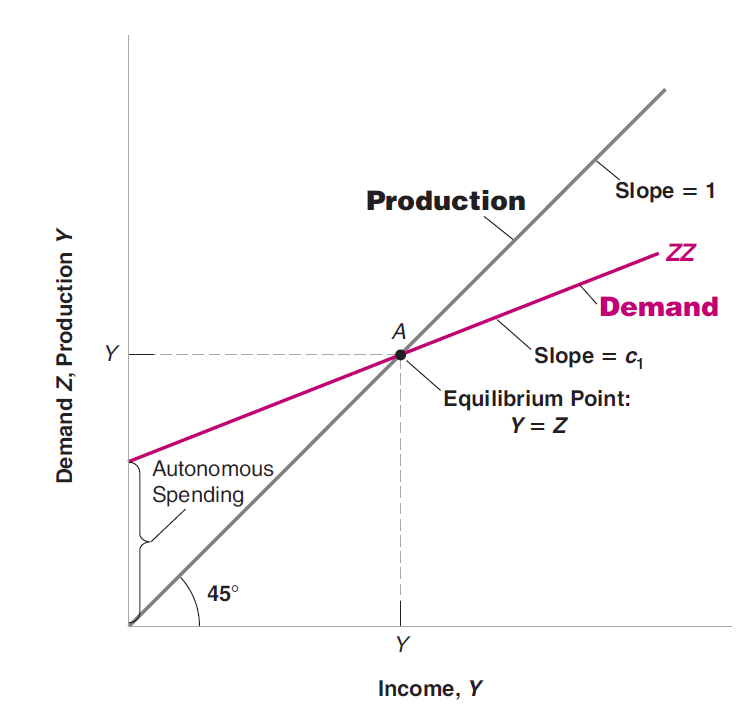
\includegraphics[width=1\textwidth]{3_1} %插入图片,[]中设置图片大小,{}中是图片文件名
	\caption{Equilibrium in the
		Goods Market} %最终文档中希望显示的图片标题
	\label{Fig.main2} %用于文内引用的标签
\end{figure}

纵轴为生产,横轴为收入,生产等于收入,因此其关系是$ 45^{\circ} $线
,其斜率为1。

\hspace*{\fill}

生产等于需求,需求的表达式为:

\[
Z=(c_0+\overline{I}+G-c_1T)+c_1Y
\]

需求取决于自主支出和收入——通过对消费的影响。需求与收入的关系为ZZ线。纵轴的截距等于自主性支出。ZZ线的斜率是边际消费倾向$ c_1 $。


\subsection{文字角度}
产出取决于需求,需求取决于收入,收入自身等于产出。需求增加,比如政府支出增加,导致生产以及相应的收入增加。收入增加导致需求的进一步增加,需求的增加又进一步导致生产增加,等等。




\subsection{产出调整需要多长时间?}
根据前面的假设:产出总是等于需求。产出对需求的反应是瞬时完成的。

现实的产出调整时间长短取决于企业如何修改其产出计划,以及修改计划的频度。企业越经常地调整其产出计划,而且产出对过去需求增加的反应越大,调整过程越快。

另一方面,需求的下降会导致产出的下降。

\section{投资等于储蓄:考虑商品市场均衡的另一种方法}
储蓄=私人储蓄+公共储蓄

私人储蓄(private saving, S)即消费者的储蓄,等于可支配收入减去消费:
\[
S\equiv Y_D-C
\]
\[
S\equiv Y-T-C
\]

根据定义公共储蓄(public saving)等于税收(减去转移支付)减去政府支出,T-G。

如果税收超过 政府支出,政府持有财政盈余(budget surplus),因此公共储蓄为正。如果税收少于政府支出,政府持有财政赤字(budget deficit),因此公共储蓄为负。

\begin{equation*}
	\begin{split}
	Y&=C+I+G\\
	Y-T-C&=I+G-T\\
	S&=I+G-T\\
	I&=S+(T-G)
	\end{split}
\end{equation*}
投资等于私人储蓄+公共储蓄,因此产品市场均衡条件也被叫作IS关系。

产品市场均衡条件的两种等价表述方法:

产出=需求

投资=储蓄

\hspace*{\fill}

推导:
\begin{equation*}
	\begin{split}
	S=Y-T-C&=Y-T-c_0-c_1(Y-T)\\
	&=-c_0+(1-c_1)(Y-T)
	\end{split}
\end{equation*}
其中$ (1-c_1) $为边际储蓄倾向。

代入IS条件:
\[
I=-c_0+(1-c_1)(Y-T)+(T-G)
\]
得到产出:
\[
Y=\frac{1}{1-c_1}[c_0+\overline{I}+G-c_1T]
\]

\hspace*{\fill}

储蓄悖论(saving paradox):

根据均衡条件:

\[
I=S+(T-G)
\]

按照假定,投资不会变:$ I=\overline{I} $,T、G也不会变。因此均衡等式告诉我们,均衡条件下,私人储蓄S也不会变。虽然人们想要在收入一定时增加储蓄,但他们的收入减少了而储蓄没有变化。这就意味着人们试图增加储蓄,结果会使产出减少,而储蓄未变。

储蓄悖论仅在短期适用,鼓励储蓄的政策可能在中长期有益,但短期可能带来经济衰退。


\section{政府是万能的吗?一个警告}
短期内政府可以通过财政政策影响需求和产出。但中长期财政政策的作用没有特别巨大。

\end{document}